\documentclass[twocolumn,10pt]{asme2e}
\usepackage{graphicx}
\usepackage{hologo}
\usepackage{amsmath}
\usepackage{caption}
\usepackage{verbatim} % for comments
\usepackage[table,xcdraw]{xcolor}
\usepackage[utf8]{inputenc}
\usepackage{hyperref}
\special{papersize=8.5in,11in}

\conffullname{the ASME 2025 \vspace{1 mm}\\ International Design Engineering Technical Conferences \vspace{1 mm}\&\\ Computers and Information in Engineering Conference\vspace{1 mm}}
\confshortname{\vspace{1 mm}IDETC/CIE2025\vspace{1 mm}}
\vspace{1 mm}
\confdate{August 17-20}
\confyear{2025}
\confcity{Anahiem, California}
\confcountry{USA}
\papernum{DETC2025-XXXXX}

\title{ \vspace{-10 mm} A Multidisciplinary Design Optimization Framework for Wave-Driven Desalination Systems}
%%% first author
\author{Nate DeGoede$^1$\thanks{Corresponding Author}, Maha Haji$^1$
    \affiliation{
	$^1$Sibley School of Mechanical and Aerospace Engineering\\
	Cornell University\\
	Ithaca, New York 14853\\
    Email: \{njd76, maha\}@cornell.edu 
    }
}

\begin{document}
\maketitle

% decrease the space buffer around equations
\setlength{\abovedisplayskip}{10pt}
\setlength{\belowdisplayskip}{10pt}

\begin{abstract}

Seawater reverse osmosis (SWRO) desalination offers a critical solution to global water scarcity, but its high energy demand necessitates sustainable power sources. Wave energy converters (WECs) present a promising alternative, particularly wave-driven desalination systems (WDDS), where they directly pressurize seawater without the inefficiencies of electrical conversion. Despite this potential, high costs remain a barrier to widespread adoption. 

This study introduces a multidisciplinary design optimization (MDO) framework to enhance WDDS performance and cost-effectiveness. The framework integrates hydrodynamics, system dynamics, desalination processes, and economic modeling, enabling holistic system-level optimization.  As a precursor to full MDO, a Latin hypercube sampling (LHS) design of experiments (DOE) study is conducted to explore key design trade-offs. 

Results highlight the importance of balancing WEC, power take-off (PTO), and desalination plant sizing. Notably, traditional designs favoring large accumulators and small SWRO plants may benefit from smaller accumulators and increased SWRO plant capacity, reducing the levelized cost of water (LCOW). Feature importance analysis further identifies key parameters influencing performance, guiding future optimization. Optimization results are forthcoming and will be included in the final paper and presentation.

This study lays the groundwork for cost-effective WDDS development, demonstrating the potential of MDO methodologies to improve desalination affordability and sustainability.

\end{abstract}


\section{Introduction}

The world is facing a growing water crisis, with global freshwater demand projected to grow over 40\% by 2050 \cite{watershortage2015}. This rising demand, compounded by factors such as droughts, urbanization, and uneven distribution of water resources, will put immense stress on existing freshwater supplies. Seawater reverse osmosis (SWRO) is promising solution to mitigate this stress by providing desalinated water. However, SWRO is energy-intensive, requiring 2-4 kWh/m$^3$ \cite{Li2018}. If powered by fossil fuels, this process would further contribute to climate change, exacerbating water scarcity issues \cite{nytdrought}. Therefore, to ensure sustainability, SWRO must be powered by renewable energy sources. 

Wave Energy Converters (WECs) offer a compelling solution. Both SWRO and WECs are marine-based technologies, with SWRO plants typically located on the coast and WECs deployed offshore. Beyond this natural co-location, WECs are particularly suited for SWRO \cite{blue_econ} due to their ability to directly pressurize seawater using a hydraulic style power take-off (PTO) system, forming a wave-driven desalination system (WDDS) \cite{Davies2005}. Unlike other renewable energy sources that require energy conversion to electricity, WECs can provide direct mechanical power, improving overall efficiency. 

Despite their potential, WECs face significant economic and technical challenges, with high costs being a primary barrier to widespread adoption. Design optimization is therefore essential for reducing costs and improving performance. Multidisciplinary Design Optimization (MDO) provides a systematic framework for addressing these challenges by integrating multiple interdependent subsystems into a unified design process, allowing for global optimization rather than isolated improvements \cite{Sobieski}. MDO-style approaches integrating PTO design with hydrodynamics and/or controls have successfully enhanced electricity-generating WECs, demonstrating its potential to enhance efficiency and energy output \cite{Stroefer2023,PenaSanchez2022,Rosati2023,Grasberger2024}. For instance, Michelén Ströfer et al. (2023) achieved a 22\% increase in electrical power output using control co-design (CCD), while Grasberger et al. (2024) demonstrated a 60\% improvement in normalized power output compared to traditional sequential design methods. These studies emphasize the importance of holistic modeling, which accounts for wave dynamics, WEC operation, PTO performance, and control strategies. Although these studies have showed great promise for MDO to improve WECs, these approaches have yet to be applied to WDDS, leaving a critical gap in research. 

This study addresses this gap by developing a holistic MDO framework for WDDS. As a precursor to full optimization, a design of experiments (DOE) study is conducted to explore key system parameters and establish a foundation for optimizing freshwater production. A simplified WDDS architecture is introduced (Fig \ref{fig:WDDS}), where an oscillating surge wave energy converter (OSWEC) drives a piston pump, pressurizing seawater and delivering it to an onshore SWRO plant. The high-pressure seawater enables freshwater production without requiring external energy input. While similar systems have been studied \cite{Yu2018,Suchithra2022,Mi2023,Simmons2024}, this study excludes an energy recovery unit (ERU)---a component known to enhance efficiency---to focus on the MDO aspects of the system. A comparison between configurations with and without the ERU will be the topic of future work.

\begin{figure}[b!]
    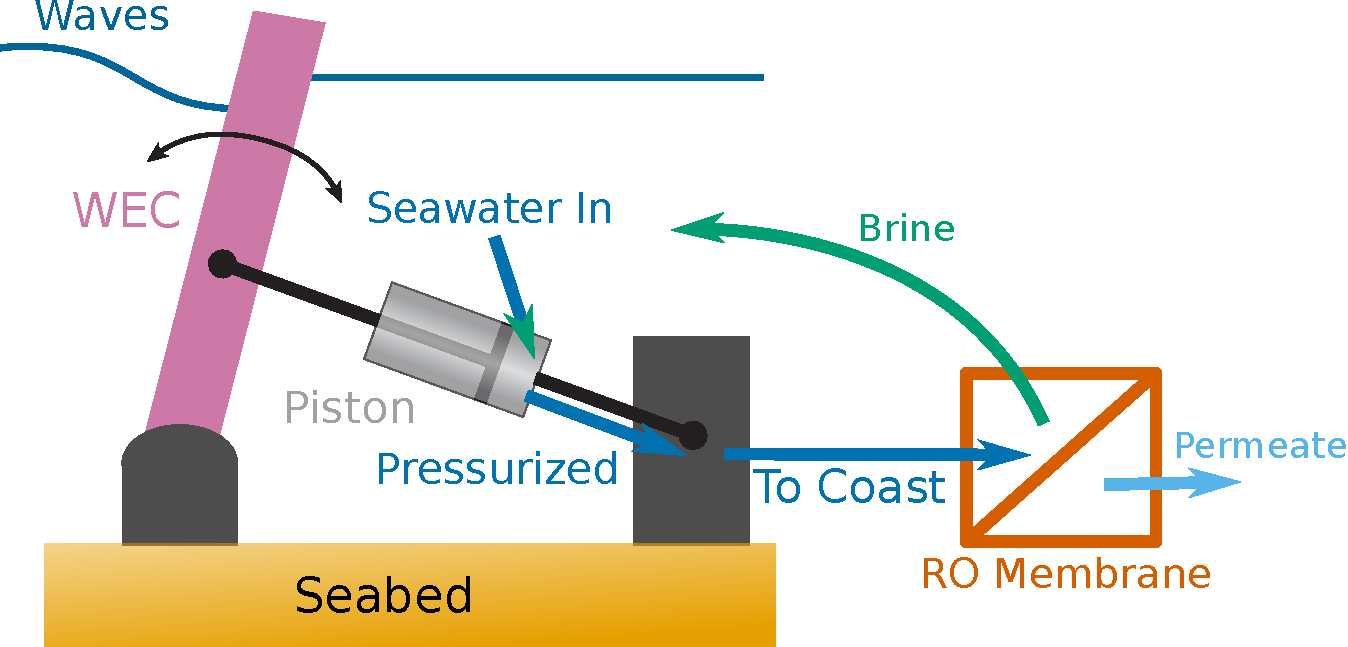
\includegraphics[width=\linewidth]{../figs/wdds.pdf}
    \captionof{figure}{Simple wave-driven desalination system (WDDS) concept Sketch.}
    \label{fig:WDDS}
\end{figure}

The concept sketch in Fig \ref{fig:WDDS} provides an overview of the WDDS but does not depict all hydraulic components included in this study. Key elements such as the hydraulic accumulator, pressure relief valve, brine side throttle valve, and directional control valves are omitted for simplicity. A detailed hydraulic circuit diagram, including these components, is show in Fig \ref{fig:hydraulics}.

\begin{figure}[t!]
    \centering
    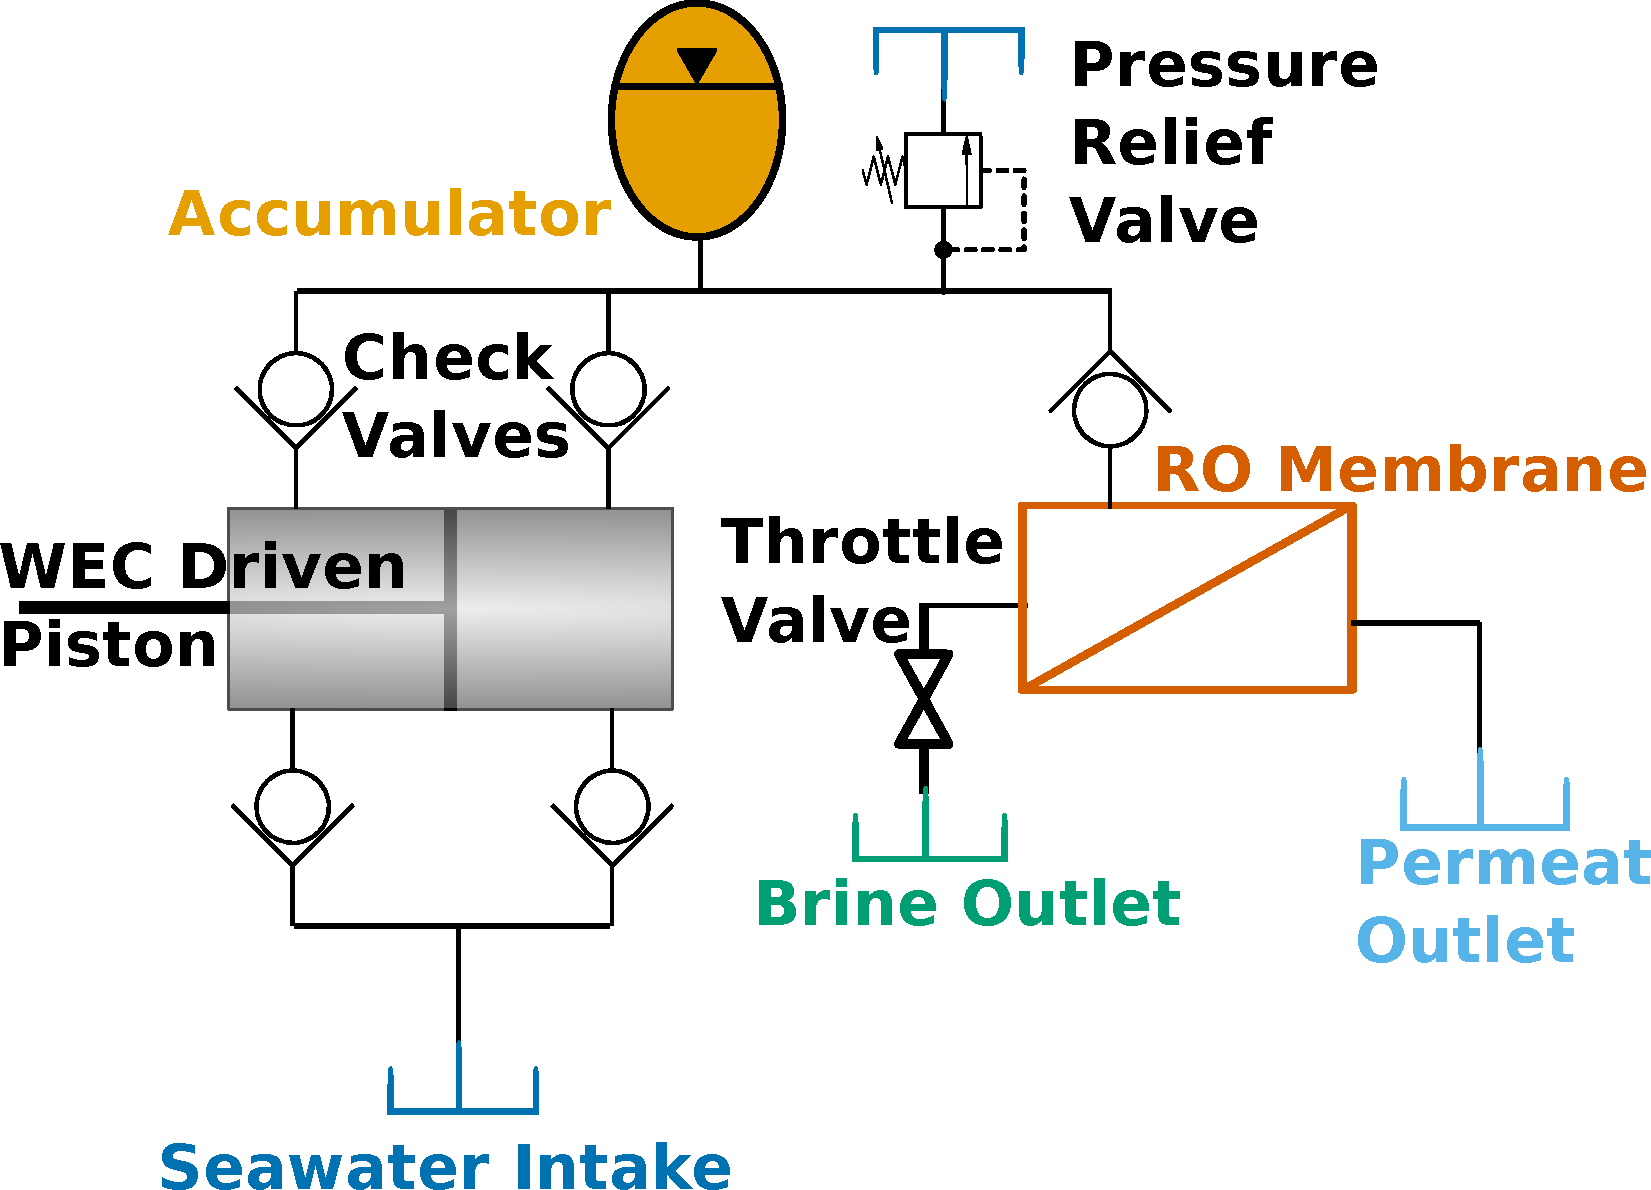
\includegraphics[width=0.7\linewidth]{../figs/hydraulic_circuit.pdf}
    \captionof{figure}{Hydraulic circuit diagram of the WDDS.}
    \label{fig:hydraulics}
\end{figure}

The following sections present the MDO problem formulation, defining the design variables that shape the design space. A comprehensive WDDS model is then introduced, structured into key modules: desalination plant, hydrodynamics, system dynamics, and economic analysis. Finally a DOE is conducted to illustrate the potential design insights that full optimization could provide. Full optimization results are forthcoming and will be included in the final paper and presented at the conference.

All code for this study can be accessed at \href{https://github.com/symbiotic-engineering/mdo_wd2}{https://github.com/symbiotic-engineering/mdo\_wd2}.

\section{Problem Formulation}
\subsection{Multidisciplinary Design Optimization Framework}
The optimization problem in this study is formally defined as:
\begin{align*} 
    \text{Minimize} \quad & \text{LCOW}(\mathbf{x},\mathbf{p}; \hat{u})  \\
    \text{by varying} \quad & \mathbf{x}\\
    \text{subject to } \quad &  \mathbf{g} \leq 0 \\
                             &  \mathbf{h} = 0 \\
                            % &  C_1 = |\mathbb{E}(j\omega)| - (A + \frac{h}{2})  \leq 0 \\
    \text{while solving} \quad & \mathbf{R}(\mathbf{x},\mathbf{p};\hat{u}) = 0\\
    \text{for } \quad & \hat{u}
    \label{eq:problem}
\end{align*}
\noindent where LCOW (levelized cost of water) is the objective function to be minimized (further discussed in section \ref{sec:econ}), $\mathbf{x}$ represents a vector of design variables, $\mathbf{p}$ represents a vector of parameters, and $\hat{u}$ is the vector of coupled variables. The constraints include inequality constraints ($\mathbf{g} \leq 0$) and equality constraints ($\mathbf{h}=0$), while $\mathbf{R}$ represents the governing equations for different disciplinary modules. The different disciplines represented in this framework are seawater desalination, hydrodynamics, system dynamics, and economics, and are discussed further in the system modeling section (Section \ref{sec:sysmodel}). Controls are not included at this time, but will be included in future work.

\subsection{Design Space}
The design vector, $\mathbf{x}$, consists of the following variables: WEC width, $w$ [m], WEC thickness, $t$ [m], WEC mass, $m$ [kg], the distance from the WEC hinge to the PTO joint, $\ell_1$ [m], piston area, $A_p$ [m$^2$], accumulator volume, $V_{acc}$ [m$^3$], accumulator pre-charge pressure, $P_0$ [MPa], and SWRO plant capacity, $Q_{p,max}$ [m$^3$/day]. Table \ref{tab:design_space} summarizes the design variables, their bounds and nominal values. Some of the key WEC dimensions are shown in Fig. \ref{fig:dims}.
\begin{table}[h]
    \centering
    \caption{Design variables}
    \begin{tabular}{|c|c|c|c|}
        \hline
        Variable & Nominal Value & Lower Bound & Upper Bound\\
        \hline
        $w$ & 18 m & 10 m & 30 m \\
        $t$ & 2 m & 1 m & 5 m \\
        $m$ & 127$\times10^3$ kg & 50$\times10^3$ kg & 500$\times10^3$ kg \\
        $\ell_1$ & 2 m & 0.1 m & draft \\
        $A_p$ & 0.26 m$^2$ & 0.01 m$^2$ & 1 m$^2$ \\
        $V_{acc}$ & 4 m$^3$ & 0.01 m$^3$ & 6 m$^3$ \\
        $P_0$ & 3 MPa & 1 MPa & 7 MPa \\
        $Q_{p,max}$ & 3150 m$^3$/day & 1000 m$^3$/day & 10000 m$^3$/day\\
        \hline
    \end{tabular}
    \label{tab:design_space} 
\end{table}

One notable aspect of the bounds is that the upper bound of $\ell_1$ is set to the draft parameter rather than a fixed value. The draft represents the distance from the still water line to the bottom of the WEC float. The WEC width refers to the sway dimension, while the WEC thickness corresponds to the surge dimension. To reduce the dimensionality of the design space, draft and height are excluded as design variables, as the chosen variables already provide sufficient control WEC dynamics. The WEC dimensions are illustrated in Fig. \ref{fig:dims}. Additionally, to aid in the interpretation of $\ell_1$, a mechanism diagram is provided in Fig. \ref{fig:mechanism}, which also shows the intakes location defined by $\ell_2$ and $\ell_3$ (both of which are parameters rather than design variables).

\begin{figure}
    \centering
    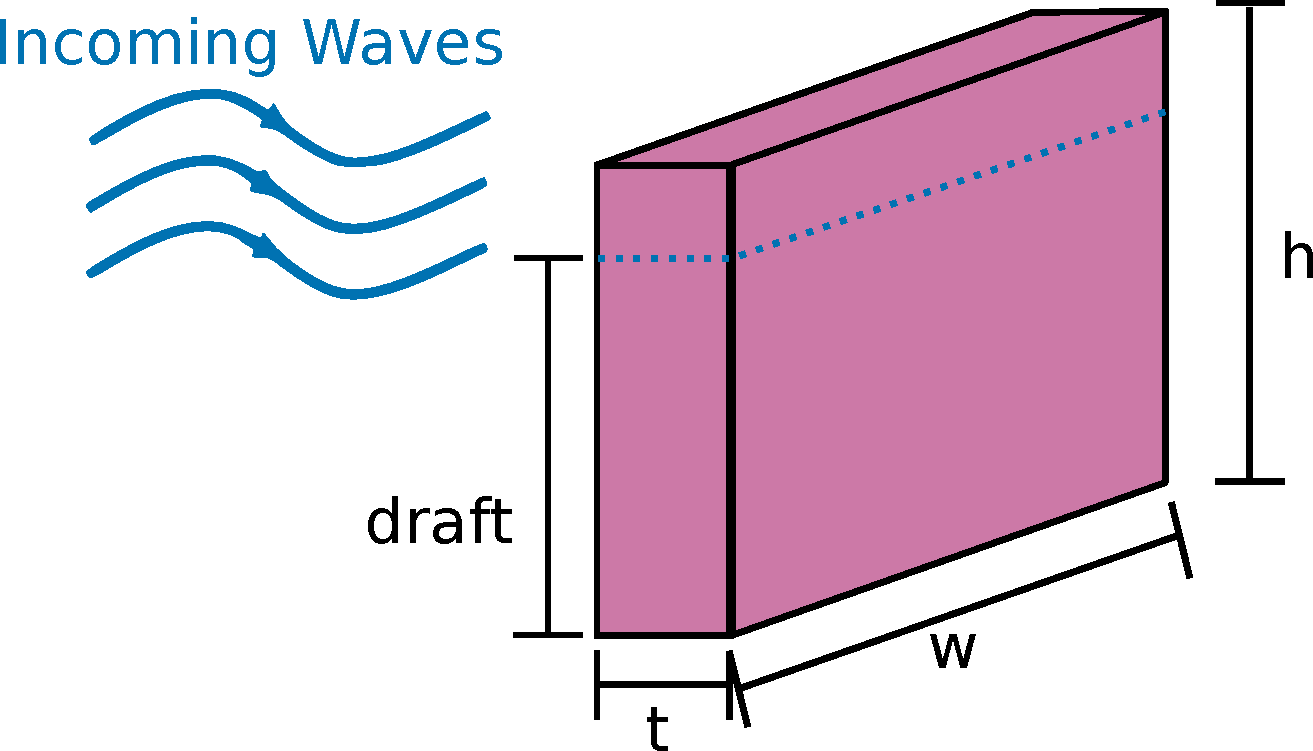
\includegraphics[width=0.7\linewidth]{../figs/WECdims.pdf}
    \captionof{figure}{WEC Dimensions. Note that $h$ represents the WEC height, which is a parameter rather than a design variable.}
    \label{fig:dims}
\end{figure}

\begin{figure}
    \centering
    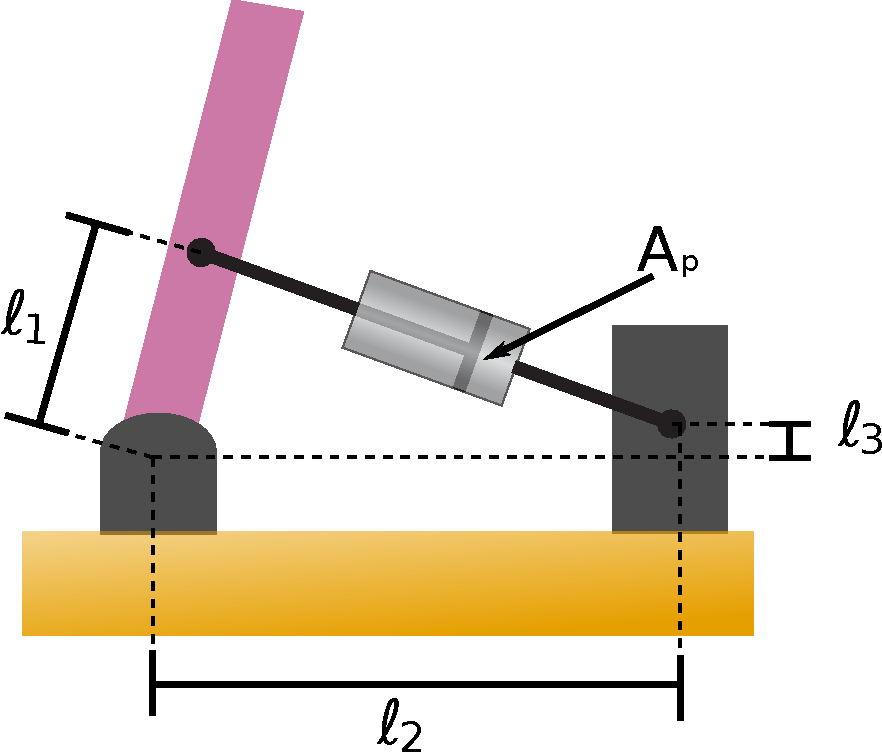
\includegraphics[width=0.7\linewidth]{../figs/mechanism.pdf}
    \captionof{figure}{Mechanism Diagram.}
    \label{fig:mechanism}
\end{figure}

\subsection{Parameters and Constraints}
Parameters were largely reflect the parameters used by Yu and Jenne (2018) \cite{Yu2018}. The subcategories of parameters include: general (parameters like gravity and wave conditions), desalination, WEC, mechanism, and solver parameters for the different submodules. Full tables of parameters can be found in appendix \ref{app:params}.

Constraints are largely enforced by the system dynamics module (Section \ref{sec:sysdyn}). These constraints are applied to constrain piston motion, ensure SWRO plant is not operated above capacity, and to ensure force and energy balance within the system.

\subsection{Optimization Algorithm}
A genetic algorithm (GA) is the most suitable choice for this problem due to the absence of accessible gradients in the hydrodynamics (Section \ref{sec:hydro}) and system dynamics (Section \ref{sec:sysdyn}) modules. While finite differencing these modules is theoretically possible, these modules are highly computationally expensive, making such an approach impractical. Consequently, a heuristic algorithm like a GA is the best choice. Optimization results are forthcoming and will be included in the final paper and presented at the conference. 

\section{System Modeling} \label{sec:sysmodel}
The system model is depicted in the N$^2$ Diagram in Fig. \ref{fig:n2}, illustrating the relationships between different disciplinary modules. Arrows represent data flow between modules, showing interdependence across the system. The model consists of four primary modules: ``Desal", which calculates dependent variables related to the SWRO plant, ``Hydro", which calculates dependent variables related to the wave-structure interaction, ``SysDyn" which solves the system dynamics of the WDDS, and ``Econ" which evaluates the LCOW objective. Additionally, a ``Mapper" module is included to map variables and parameters to dependent variables across different modules. However, since it does not contribute to independent disciplinary calculations, it is not considered a separate discipline. The four main modules are discussed in more detail in the following subsections. 

\begin{figure}
    \centering
    \includegraphics[width=0.7\linewidth]{../figs/n2.pdf}
    \captionof{figure}{N$^2$ Diagram of the WDDS System Model.}
    \label{fig:n2}
\end{figure} 

\subsection{Desalination Module}
The desalination module calculates key parameters for the SWRO plant, considering the system's capacity and seawater composition. The reverse osmosis process is governed by:
\begin{equation}
    \label{eq:ro}
    Q_p = A_w A_m (\Delta P - \Delta \pi)
\end{equation}
\noindent where $Q_p$ [m$^3$/s] is the permeate flow rate, $A_w$ [m$^2$] is the water permeability coefficient, $A_m$ [m$^2$] is the membrane area, $\Delta P$ [Pa] is the pressure difference across the membrane, and $\Delta \pi$ [Pa] is the osmotic pressure difference across the membrane. The osmotic pressure is calculated using \cite{separationprocesses}:
\begin{equation}
    \label{eq:osmotic_pressure}
    \pi = iCRT
\end{equation}
\noindent where $i$ [-] is the number of ions produced per molecule of solute, $C$ [mol/m$^3$] is the concentration of the solute, $R$ [J/K-mol] is the ideal gas constant, and $T$ [K] is the temperature.

For seawater applications, Applegate's empirical formula \cite{separationprocesses} provides an alternative method for calculating osmotic pressure:
\begin{equation}
    \label{eq:osmotic_pressure_applegate}
    \pi = 1.12 T \sum m_i
\end{equation}
\noindent where $\sum m_i$ [mol/m$^3$] represents the sum of dissolved ion molarities. In this study, we use Eq. \ref{eq:osmotic_pressure} as our primary method. Eq. \ref{eq:osmotic_pressure_applegate} is provided as an alternative where precise seawater composition data is available. In this study, we set $\Delta \pi$ to the osmotic pressure of the seawater minus the target permeate osmotic pressure.

For the water permeability coefficient ($A_w$) we adopt the constant value of $2.57\times10^{-12}$ m$^3$/N-s, as reported by Yu and Jenne (2018) \cite{Yu2018}. This choice is justified by our use of the same SWRO membrane, the SW30HR-380 Dry from DuPont \cite{SW30HR380}, for which their coefficient was determined. The membrane area $A_m$ is then given by
\begin{equation}
    A_m = \frac{Q_{p,max}}{Q_0}A_0
    \label{eq:membrane_area}
\end{equation}   
\noindent where $Q_0$ and $A_0$ are the nominal flow rate and membrane area for the SW30HR-380 membrane, found on the datasheet \cite{SW30HR380}.

At this stage, Eq. \ref{eq:ro} relates only pressure and flow rate. To integrate this relationship into system dynamics, we define the membrane resistance ($R_m$ [MPa-s/m$^3$] ) as:
\begin{equation}
    \frac{1}{A_w A_m}
    \label{eq:membrane_resistance}
\end{equation}
\noindent This allows for a linearized resistance model, simplifying system-level calculations.

To avoid running the system above capacity, a pressure relief valve is included, with its set pressure $P_{\text{relief}}$ [MPa] defined as:
\begin{equation}
    P_{\text{relief}} = Q_{p,max}R_m + \Delta \pi
    \label{eq:pressure_relief}
\end{equation}

This equation ensures that if the flow exceeds the system's capacity, the pressure relief valve will open. Notably, by combining Eqs. \ref{eq:membrane_area} \ref{eq:membrane_resistance} and \ref{eq:pressure_relief}, the dependency on $Q_{p,max}$ cancels out, making $P_{\text{relief}}$ independent of specific design parameters under the current membrane resistance model. However, this remains a dependent variable, allowing for flexibility in alternative design spaces or resistance models.

For flow to pass through the membrane, resistance on the brine side is required. This can achieved using a throttle valve (as modeled in this study), or an ERU (for higher efficiency in advanced designs). In this study we implement a constant throttle valve resistance ($R_t$ [MPa-s/m$^3$]), calculated such that when the system runs at full capacity, it also runs at the recommended recovery ratio, $\eta_{RO}$, given the SW30HR-380 membrane and the specified seawater composition.
\begin{equation}
    R_t = \frac{P_{\text{relief}}}{Q_{p,max}(\frac{1}{\eta_{RO}} - 1)}
\end{equation}

\subsection{Hydrodynamics} \label{sec:hydro}
Starting from Newton's second law, Falnes and Kurniawan (2022) \cite{falnes2022} define the equation of motion for an oscillating WEC as:
\begin{equation}
    \label{eq:cummins}
    I\ddot{\xi} = f_e - f_r - f_b - f_v - f_f - f_u  
\end{equation}
\noindent where $I$ [m or kg-m$^2$] is the inertia of the WEC, dependent on WEC mass $m$ (a design variable), $\xi$ [m or rad] is the body linear or angular motion, $f_e$ [N or Nm] is the excitation force or torque due to incident waves, $f_r$ [N or Nm] is the radiation force or torque due to the WEC’s oscillations, accounting for added mass and radiation damping, $f_b$ [N or Nm] is the hydrostatic force or torque due to buoyancy and restoring effects, $f_v$ [N or Nm] is the drag force or torque which arises from nonlinear viscous effects (neglected in this study), $f_f$ [N or Nm] is the force or torque that captures friction forces (also neglected), and $f_u$ [N or Nm] is the PTO force or torque, which represents energy extraction by the WEC’s power conversion system. The PTO force is modeled in the system dynamics module, while drag and friction are omitted, assuming linear potential flow theory. These simplifications are also made by Grasberger et al. (2024) \cite{Grasberger2024} in their OSWEC study. 

The hydrostatic force, which accounts for the buoyancy of the WEC and its tendency to return to equilibrium, is given by: 
\begin{equation}
    \label{eq:hydrostatic}
    f_{hs} = K_{hs} \xi
\end{equation}
\noindent where $K_{hs}$ is the hydrostatic stiffness matrix.

The radiation force, which accounts for the radiated waves generated by the WEC motion, is expressed as:
\begin{equation}
    \label{eq:radiation}
    f_r = A(\omega) \ddot{\xi} + B(\omega) \dot{\xi}
\end{equation}
\noindent where $A(\omega)$ and $B(\omega)$ are the added mass and radiation damping matrices, respectively.

This formulation simplifies the WEC hydrodynamics to four key components: the excitation force, hydrostatic stiffness matrix, added mass matrix, and radiation damping matrix. These coefficients are computed using the open-source Boundary Element Method (BEM) solver Capytaine \cite{ancellin_capytaine_2019}. BEM solvers are well suited for wave-structure interaction problems as they only require meshing of the structure-fluid boundary, unlike traditional computational fluid dynamics (CFD) solvers which require full fluid volume meshing, significantly reducing computational cost \cite{bem_wave}.

For this study, the WEC flap is approximated as a rectangular prism, restricted to pitch motion about its bottom hinge. Notably, added mass, radiation damping, and excitation force are all frequency-dependent.

%The added mass and radiation damping matrices are calculated by sweeping across frequencies and solving Capytaine's radiation problem. The excitation force is calculated by sweeping across frequencies and solving Capytaine's diffraction problem and then combining the diffraction and Froude-Krylov forces. The hydrostatic stiffness is calculated using Capytaine's hydrostatics solver. These results are then used in the system dynamics module to calculate the motion of the WEC coupled with the PTO.

\subsection{System Dynamics} \label{sec:sysdyn}

The WDDS system dynamics are modeled in MATLAB+Simulink, capturing the interactions between the WEC and PTO system. The following sections detail the modeling of each subsystem.

\subsubsection{Wave Energy Converter}

The WEC dynamics are modeled using WEC-Sim \cite{wecsim}, an open-source software developed by the National Renewable Energy Laboratory (NREL) and Sandia National Laboratories. Using hydrodynamic coefficients obtained from the hydrodynamics module, WEC-Sim simulates WEC system dynamics within a Simulink-based framework, enabling efficient analysis of wave-structure interactions and PTO performance. WEC-Sim offers significant advantages over other WEC simulation tools by operating in the time domain, allowing it to capture complex dynamics and nonlinearities that many alternative methods can only approximate. The WEC is modeled as a two body system, with the base fixed to the seafloor and the flap limited to a one degree of freedom (pitch). The WEC model also includes the mechanism to drive the piston. With the intake location, hinge location, and PTO joint location all defined according to Fig. \ref{fig:mechanism}. The block diagram used to model the WEC is shown in Fig. \ref{fig:wec_simscape}.

\begin{figure}[b!]
    \includegraphics[width=\linewidth]{../figs/wecsimscape.pdf}
    \captionof{figure}{Model of the WEC in Simscape.}
    \label{fig:wec_simscape}
\end{figure}

\subsubsection{Power Take-Off}

The desalination hydraulic circuit (Fig \ref{fig:hydraulics}) is modeled using the isothermal liquid domain from the Simscape fluids toolbox. This domain is specialized for modeling hydraulic systems, and is a good fit for modeling the dynamics of the hydraulic circuit presented. The high level Simscape PTO model is shown in Fig. \ref{fig:hydraulic_simscape}.

\begin{figure*}[t]  % The [t] option places the figure at the top of the page
    \centering
    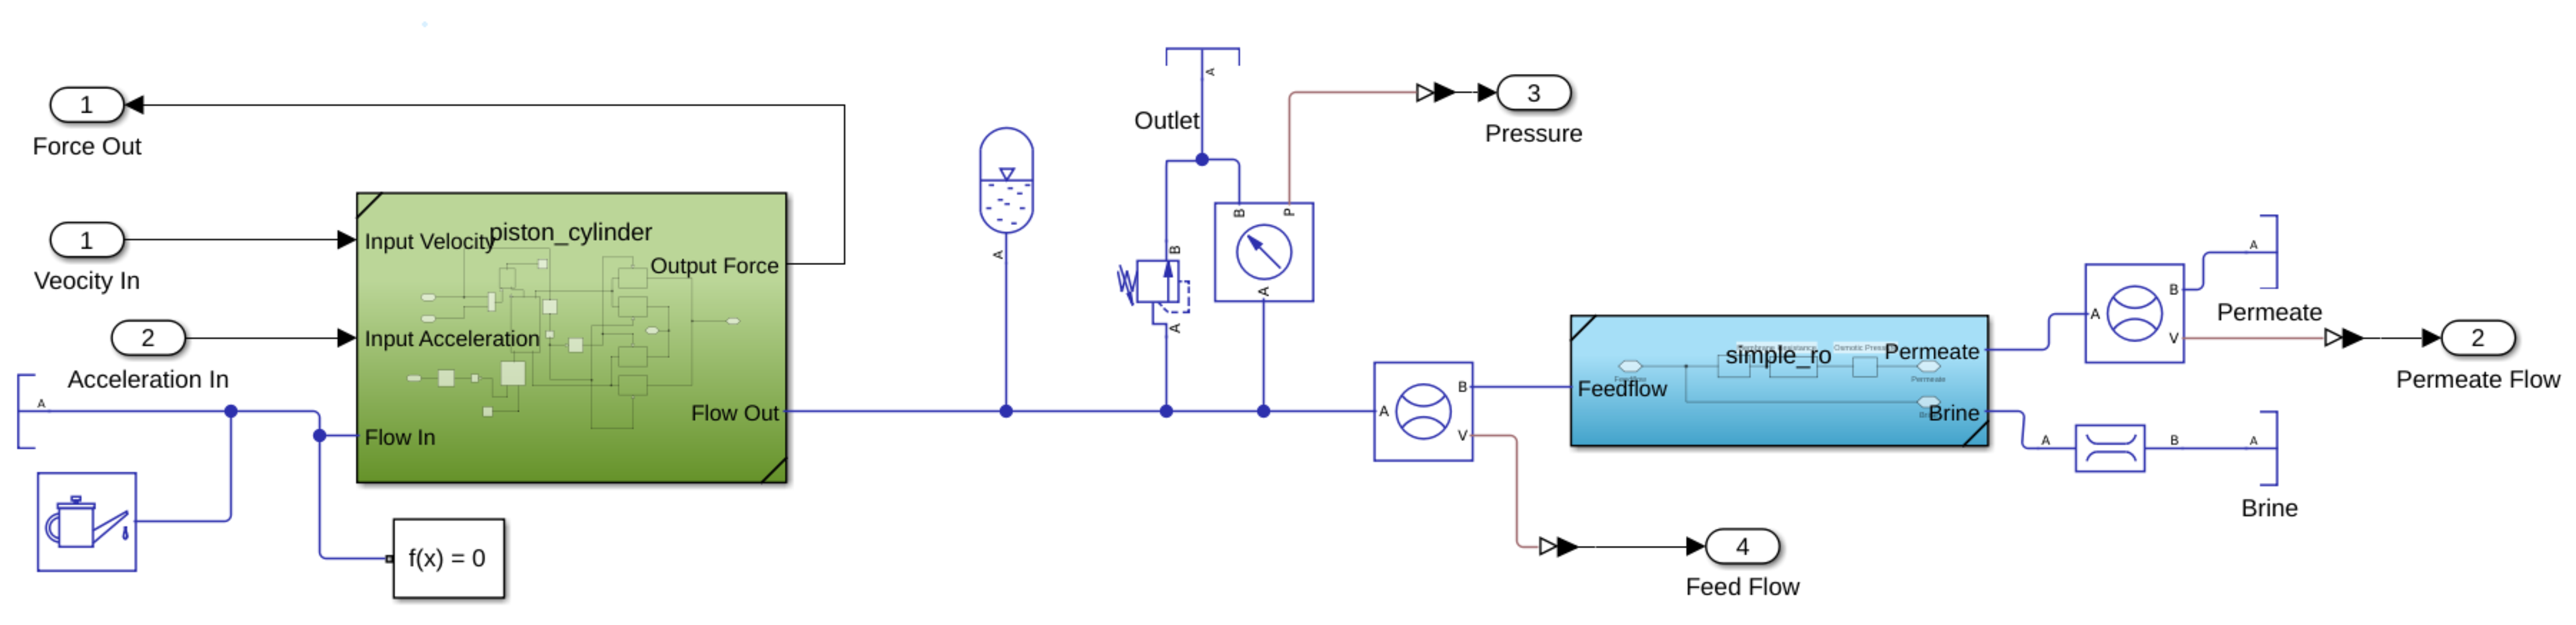
\includegraphics[width=0.8\linewidth]{../figs/hydraulic_simscape.pdf}
    \captionof{figure}{Model of the hydraulic circuit in Simscape.}
    \label{fig:hydraulic_simscape}
\end{figure*}

From this high level view, we can see the main components of the hydraulic circuit. The ``piston\_cylinder" block contains the piston and directional valves, followed by the accumulator and pressure relief valve, as well as the reverse osmosis membrane, modeled in the ``simple\_ro" block, and finally the throttle valve on the brine side.

The ``piston\_cylinder" subsystem is further broken down in Fig. \ref{fig:piston_simscape}. This model features a single double-acting piston, though the system dynamics would remain largely unchanged if the piston area variable was distributed across multiple smaller pistons instead of a single large one. Another feature of note is the use of three-way controlled directional valves instead of check valves to simplify computations for the solver while maintaining the overall system dynamics.

\begin{figure}
    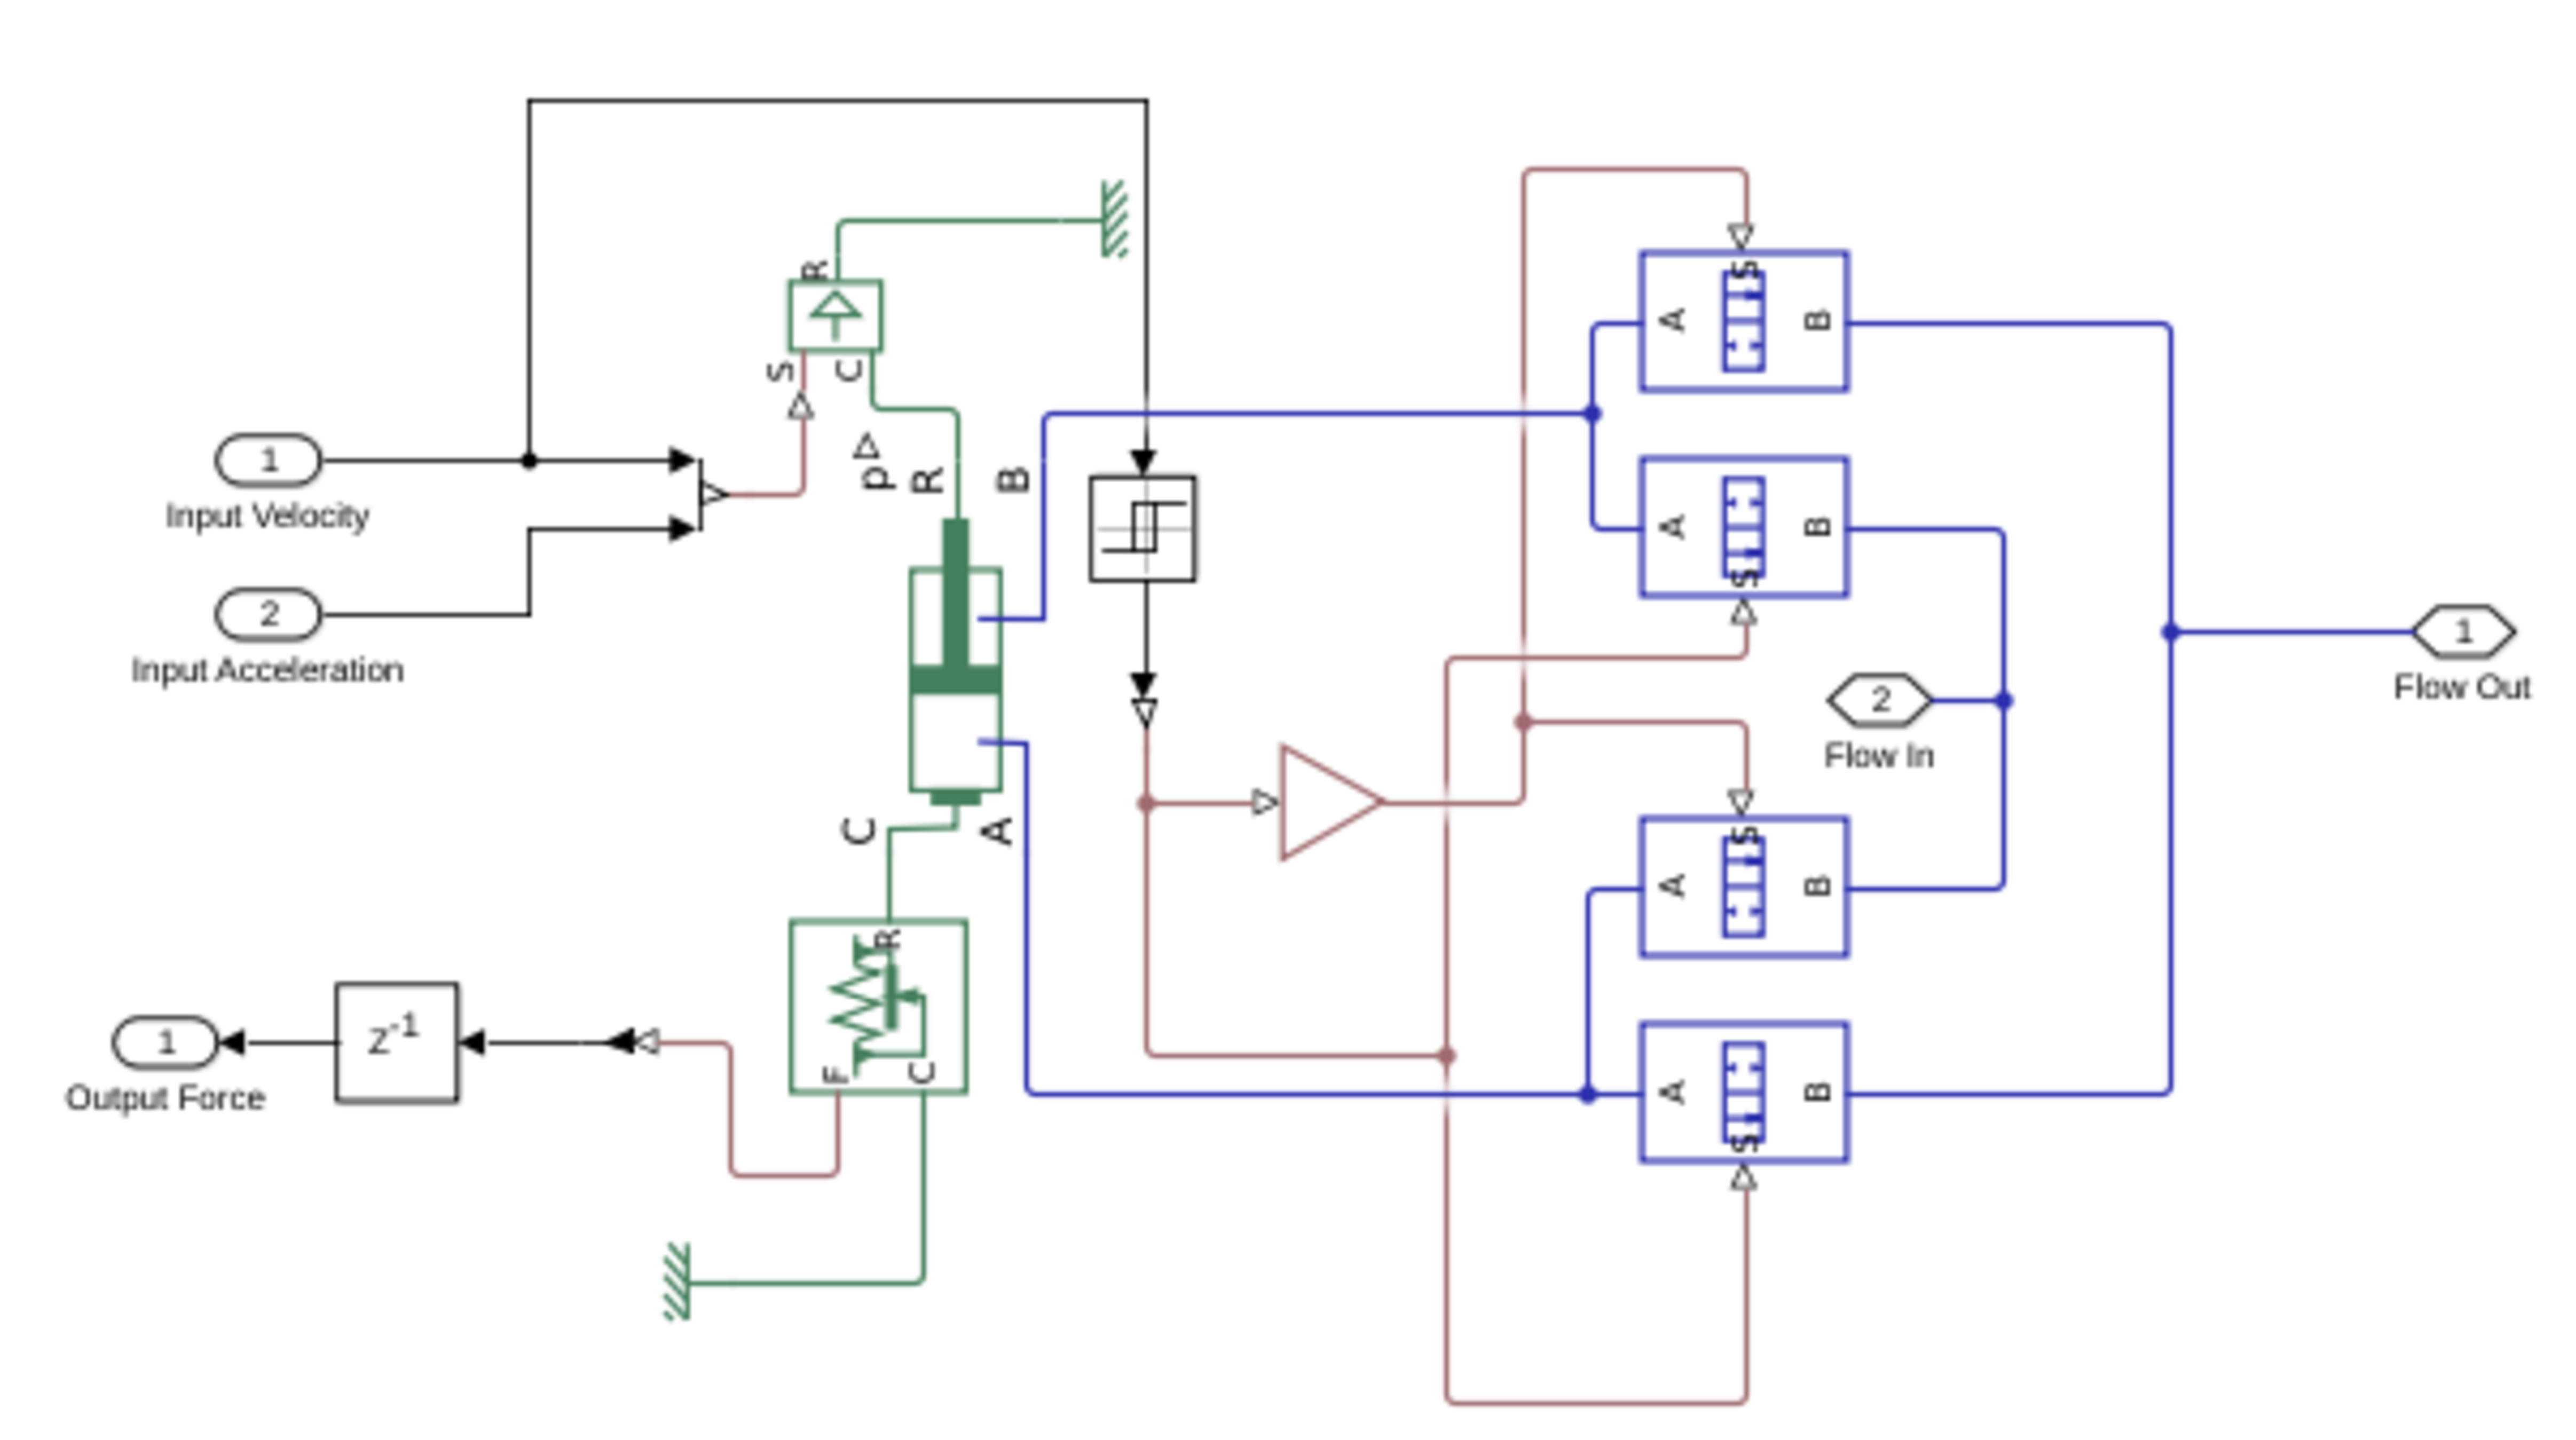
\includegraphics[width=\linewidth]{../figs/pistonsimscape.pdf}
    \captionof{figure}{Model of the piston and directional valves in Simscape.}
    \label{fig:piston_simscape}
\end{figure}

The ``simple\_ro" subsystem is broken down in Fig. \ref{fig:ro_simscape}. This subsystem includes a check valve to prevent forward osmosis in low energy waves, followed by the membrane resistance and osmotic pressure blocks which allow for a Simscape representation of eq \ref{eq:ro}. The membrane resistance block is a linear resistance on the volumetric flow rate, and the osmotic pressure block applies a pressure on the permeate side equal to the osmotic pressure difference as calculated in eqns. \ref{eq:osmotic_pressure} or \ref{eq:osmotic_pressure_applegate}.

\begin{figure}
    \centering
    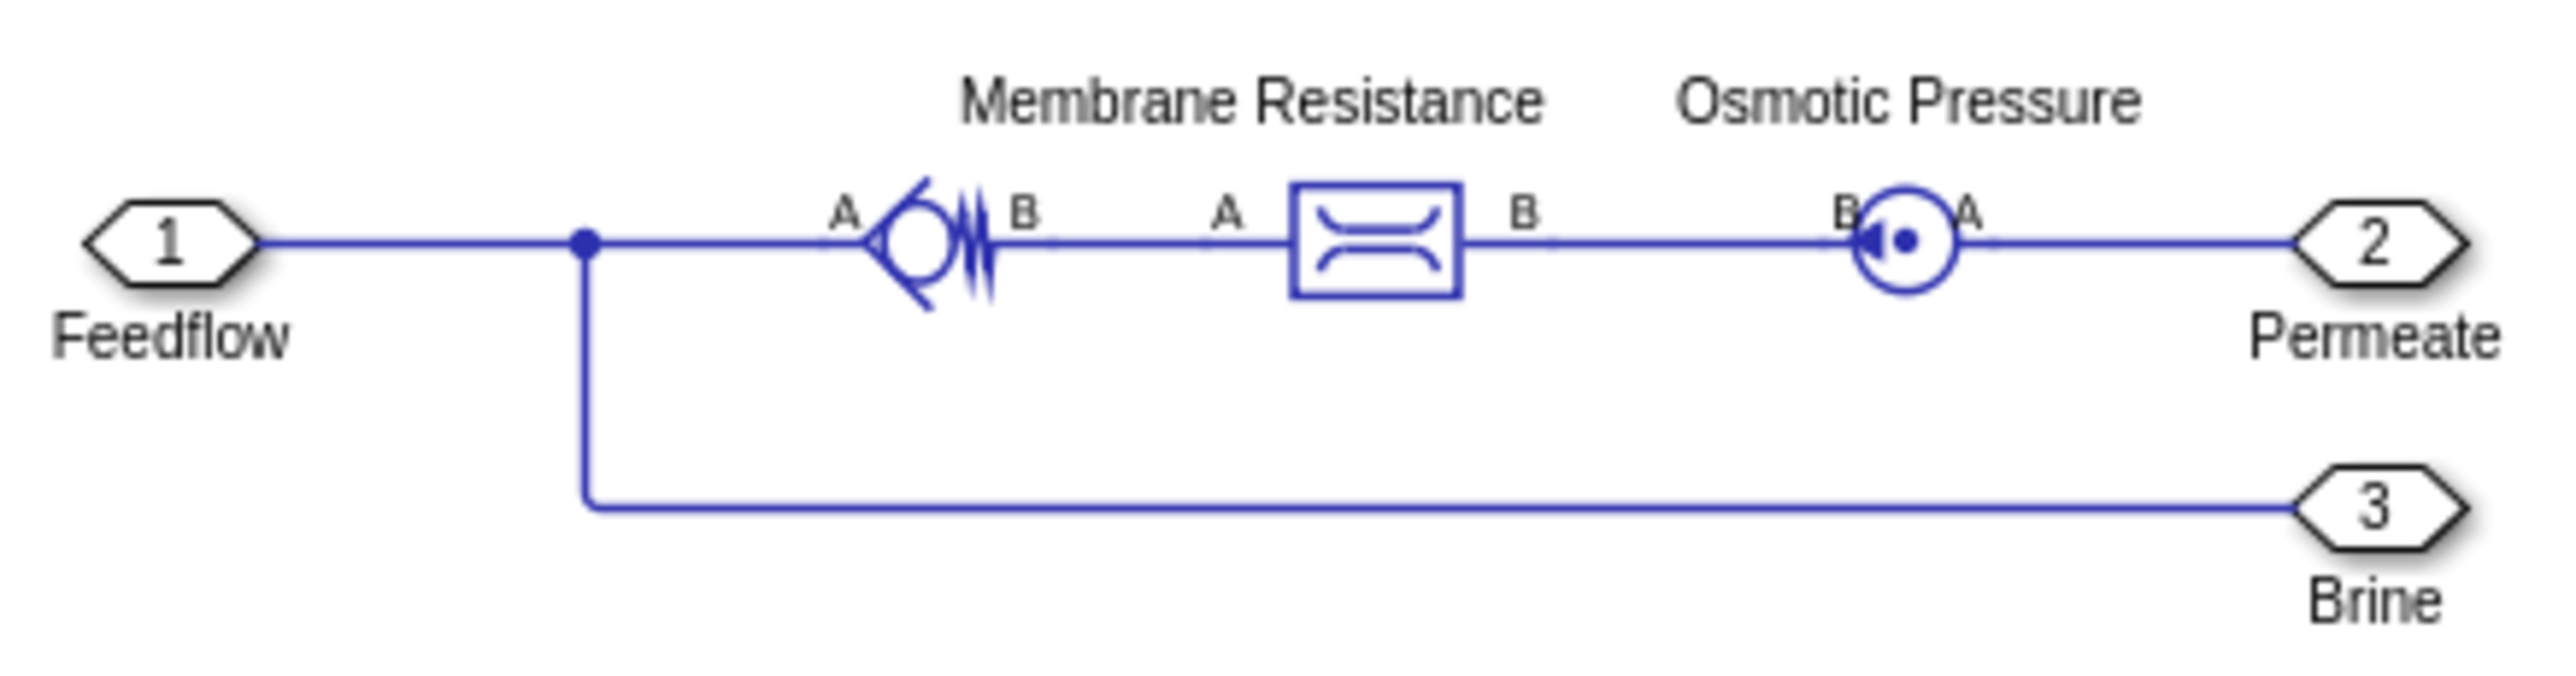
\includegraphics[width=0.8\linewidth]{../figs/desalsimscape.pdf}
    \captionof{figure}{Model of the reverse osmosis membrane in Simscape.}
    \label{fig:ro_simscape}
\end{figure}

\subsubsection{Coupled Solver}

The two subsystems of the WEC and PTO are then coupled through as shown in Fig. \ref{fig:coupled_system}. The velocity and acceleration signals are fed as inputs to the PTO from the WEC, and the force is fed back from the PTO to the WEC. WEC-Sim uses this coupled system to simulate the system dynamics of the WDDS. MATLAB's ode4 solver, a fourth order Runge-Kutta solver, with a 0.1~s time step is used to solve the system dynamics. 

\begin{figure}
    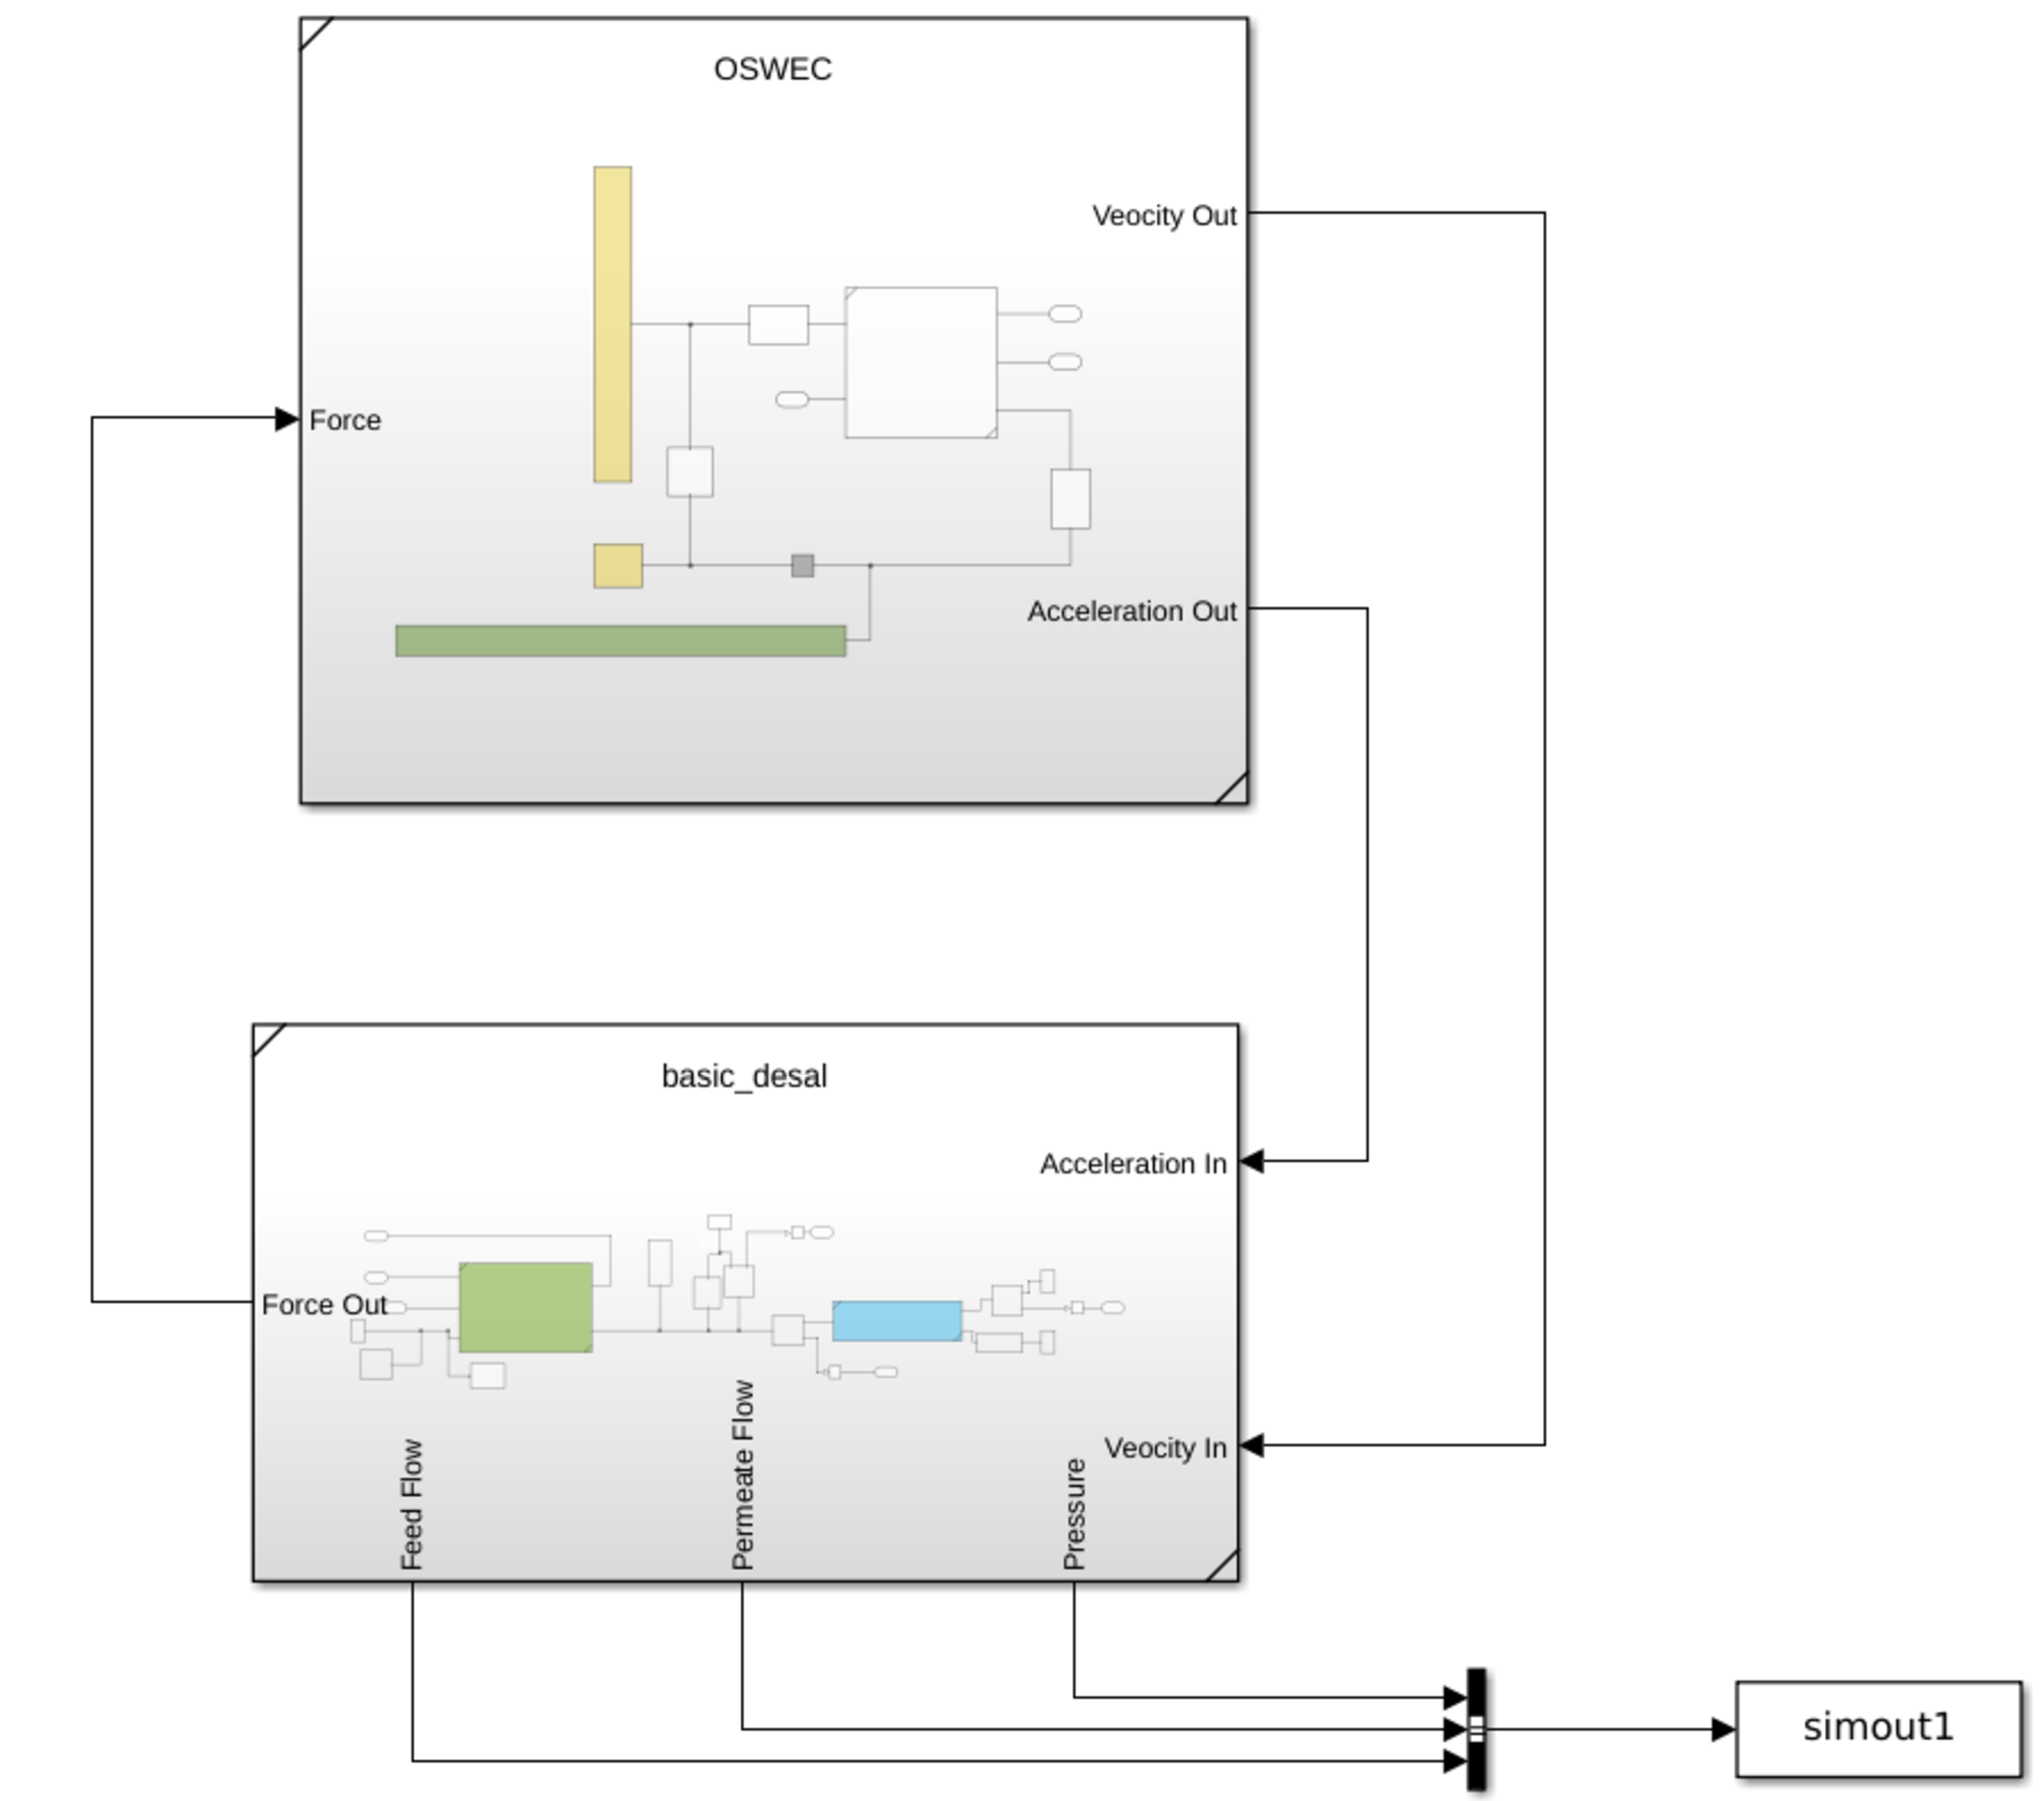
\includegraphics[width=0.8\linewidth]{../figs/coupledsimscape.pdf}
    \captionof{figure}{Model of the coupled WEC and PTO in Simscape.}
    \label{fig:coupled_system}
\end{figure}

\subsection{Economics} \label{sec:econ}

Our objective is to minimize the levelized cost of water (LCOW) [\$/m$^3$] which is calculated using the annual water production (AWP) [m$^3$/year] from the system dynamics module and the costs calculated from the economic module. We consider a simple cost model comprised of two categories: capital (CAPEX) and operational expenditures (OPEX). The LCOW is then determined by
\begin{equation}
    \text{LCOW} = \frac{(\text{FCR}\times\text{CAPEX}) + \text{OPEX}}{\text{AWP}}
    \label{eq:LCOW}
\end{equation}
\noindent where FCR is the fixed charge rate, 10.8\% based on the assumptions made in the U.S. Department of Energy report \cite{LCOE_DOE}. We note that Eq. \ref{eq:LCOW} takes a form similar to that of the levelized cost of energy (LCOE) used by the U.S. Department of Energy \cite{LCOE_DOE}. The CAPEX and OPEX are split into three sections based on the three main sections of design variables: the WEC, the PTO, and the desalination plant. It is important to note that this cost model is not meant to provide an exact representation of total system costs. Instead it serves as a tool to quantify relative cost savings between different designs, highlighting the impact of applying an MDO approach to this problem. An explanation of the cost model for each component is given below. Note that all costs are adjusted to 2025 USD.

\subsubsection{Wave Energy Converter}

Cost modeling for WECs is inherently uncertain due to limited real world data, making it difficult to achieve high accuracy. This presents a significant challenge for studies like this, where levelized cost is used as an objective function. Despite these challenges, a practical and comparative cost model can still be developed to capture key cost trends and enable design comparisons. In this study, we follow the method from Grasberger et al. (2024) who introduced a simplified cost model for their OSWEC CCD study \cite{Grasberger2024}. In this model, costs are expressed as a function of the float's surface area of the float through a combination of linear and logarithmic terms, shown below
\begin{equation}
    \text{Cost} = C_{1,ref}\left(\frac{A_{x}}{A_{ref}}\right) + C_{2,ref}\left(1 + \text{log}\left(\frac{A_{x}}{A_{ref}}\right)\right)
\end{equation}
\noindent where $A_{x}$ [m$^2$] is the surface area of the float, $A_{ref}$ [m$^2$] is the surface area of the reference float, and $C_{1,ref}$ [\$] and $C_{2,ref}$ [\$] are the costs of the reference float associated with the two terms.The linear term captures cost associated with the structural components (the flap, base, and mooring), while the logarithmic term captures other expenses (PTO, monitoring, other OPEX) which are less dependent on the size of the float. This cost model relies on an accurate reference WEC for meaningful comparisons.

Given the importance of a reliable reference WEC, we utilize NREL’s Reference Model 5 (RM5) \cite{rm5}, a well-documented OSWEC. Its similarity to the WEC design in this study makes it an appropriate benchmark for cost comparison and performance evaluation. To tailor the cost model to this study’s specific WEC design, we exclude certain cost components that are not relevant or do not scale directly with WEC size. In particular, since this design replaces an electricity-generating PTO with the a SWRO PTO, the electrical PTO costs from the initial RM5 cost model are not include. Instead, we determine SWRO PTO specific costs, detailed in the next section. Additionally, because this study considers a nearshore fixed-bottom WEC, many mooring-related expenses from the reference RM5 are not included. Finally, many transit and other overhead design costs are excluded as they are unlikely to scale proportionally with the size of the WEC. 

\subsubsection{Power Take-Off}

The PTO cost model covers the costs associated with the pumping mechanism, the piston cylinder, and the accumulator. At present, pumping mechanism and piston cylinder costs are under development and are not included in this preliminary study. Despite this exclusion, we believe the current model offers important insights into the accumulator sizing. The accumulator cost is modeled as function of the accumulator volume ($V_{acc}$). The accumulator volume design variable is rounded up to the nearest standard size based on commercially available accumulators from Reasontek \cite{reasontek} (2.5~gallons). The accumulator volume is then split into the nominal sizes available and the required amount of each size is multiplied by the quoted cost of that size. 
%A table detailing the costs of the various sizes is shown in Table \ref{tab:acc_cost}.
%\begin{table}[h]
%    \centering
%    \caption{Accumulator Costs}
%    \begin{tabular}{|c|c|}
%        \hline
%        \textbf{Volume [gal]} & \textbf{Cost [\$]} \\
%        \hline
%        2.5 & 3,985 \\
%        5 & 5,488 \\
%        10 & 7,285 \\
%        15 & 8,985 \\
%        \hline
%    \end{tabular}
%    \label{tab:acc_cost}
%\end{table}
A cost optimal accumulator configuration for a given volume is achieved when the volume is split into the as many 15~gallon accumulators as possible, followed by 10 gallon accumulators, then 5~gallon accumulators, and finally 2.5~gallon accumulators.

\subsubsection{Desalination Plant}
The costs associated with the desalination plant are divided into two categories: capital costs and operational costs. The capital costs includes all expenses related to the construction and installation of the plant, while the operational costs over the recurring costs associated with its annual operation and maintenance.

Cost models for small- to mid-scale SWRO desalination plants of this scale (producing thousands of m$^3$/day) are scares and often poorly documented or inconsistently implemented. Most well-documented economic studies focus on large-scale plants (hundreds of thousands of m$^3$/day) \cite{Slocum2016,Haefner2023,roopexcurve,Wittholz2008}, making them less applicable to this study. Meanwhile, studies that examining smaller desalination plants frequently lack transparent methodologies for estimating SWRO-specific plant costs \cite{Elkadeem2024,Goekcek2016}. One notable study on wave-driven desalination employs the Desalination Economic Evaluation Program (DEEP 5.1) developed by the International Atomic Energy Agency to estimate unit CAPEX cost \cite{Yu2022}. However, DEEP 5.1 itself is poorly documented \cite{DEEP5manual}, making it difficult to assess the accuracy and reliability of its cost estimates. 

Given these limitations, this study adopts a cost estimation methodology based on the work of Voutckov in \emph{Desalination Project Cost Estimating and Management} \cite{voutch}. Using the cost curves provided in sections 4 (CAPEX) and 5 (OPEX) of his work, a flexible cost model is developed that can be customized for different project specifications. Each curve is fitted to a power function of the form:
\begin{equation}
    y = a \cdot x^b
\end{equation}

This form was chosen because to avoid unrealistic behaviors at the lower end of the scale. Unlike polynomial fits, which can produce unrealistic negative costs, a power-law fit ensures a monotonic and physically meaningful cost relationship.

\section{Design of Experiments}
A preliminary DOE study provides valuable insights into the relative importance of design variables and relations between them and performance objectives. Additionally, DOE can help identify high-performance design configurations and establish general trends within the design space. 

For this study, we use a Latin Hypercube sampling method with 508 samples to explore the design space. The designs corresponding to minimum and maximum LCOW are presented in Table \ref{tab:doe}.
\begin{table}
    \centering
    \caption{Designs with Minimum and Maximum LCOW}
    \begin{tabular}{|c|c|c|}
        \hline
        \textbf{Variable} & \textbf{Min LCOW case} & \textbf{Max LCOW case} \\
        \hline
        $w$ & 11.5 m & 24.5 m \\
        $t$ & 4.35 m & 1.23 m \\
        $m$ & 490 $\times10^3$ kg & 139 $\times10^3$ kg \\
        $\ell_1$ & 3.11 m & 0.276 m \\
        $A_p$ & 0.932 m$^2$ & 0.394 m$^2$ \\
        $V_{acc}$ & 1.51 m$^3$ & 0.237 m$^3$ \\
        $P_0$ & 4.51 MPa & 3.92 MPa \\
        $Q_{p,max}$ & 7467 m$^3$/day & 9681 m$^3$/day \\
        \hline
        \textbf{LCOW} & 2.29 \$/m$^3$ & 7547 \$/m$^3$ \\
        \hline
    \end{tabular}
    \label{tab:doe}
\end{table}

To quantify the importance of each design variable, we employ feature importance analysis using a random forests regression model trained on the DOE dataset \cite{Rogers2006}. We compute feature importance using both mean decrease in impurity and permutation importance. These metrics indicate how much each variable contributes to predicting LCOW, helping identify potential reductions in design space complexity. The feature importance results are  shown in Fig. \ref{fig:importance}.

\begin{figure}
    \centering
    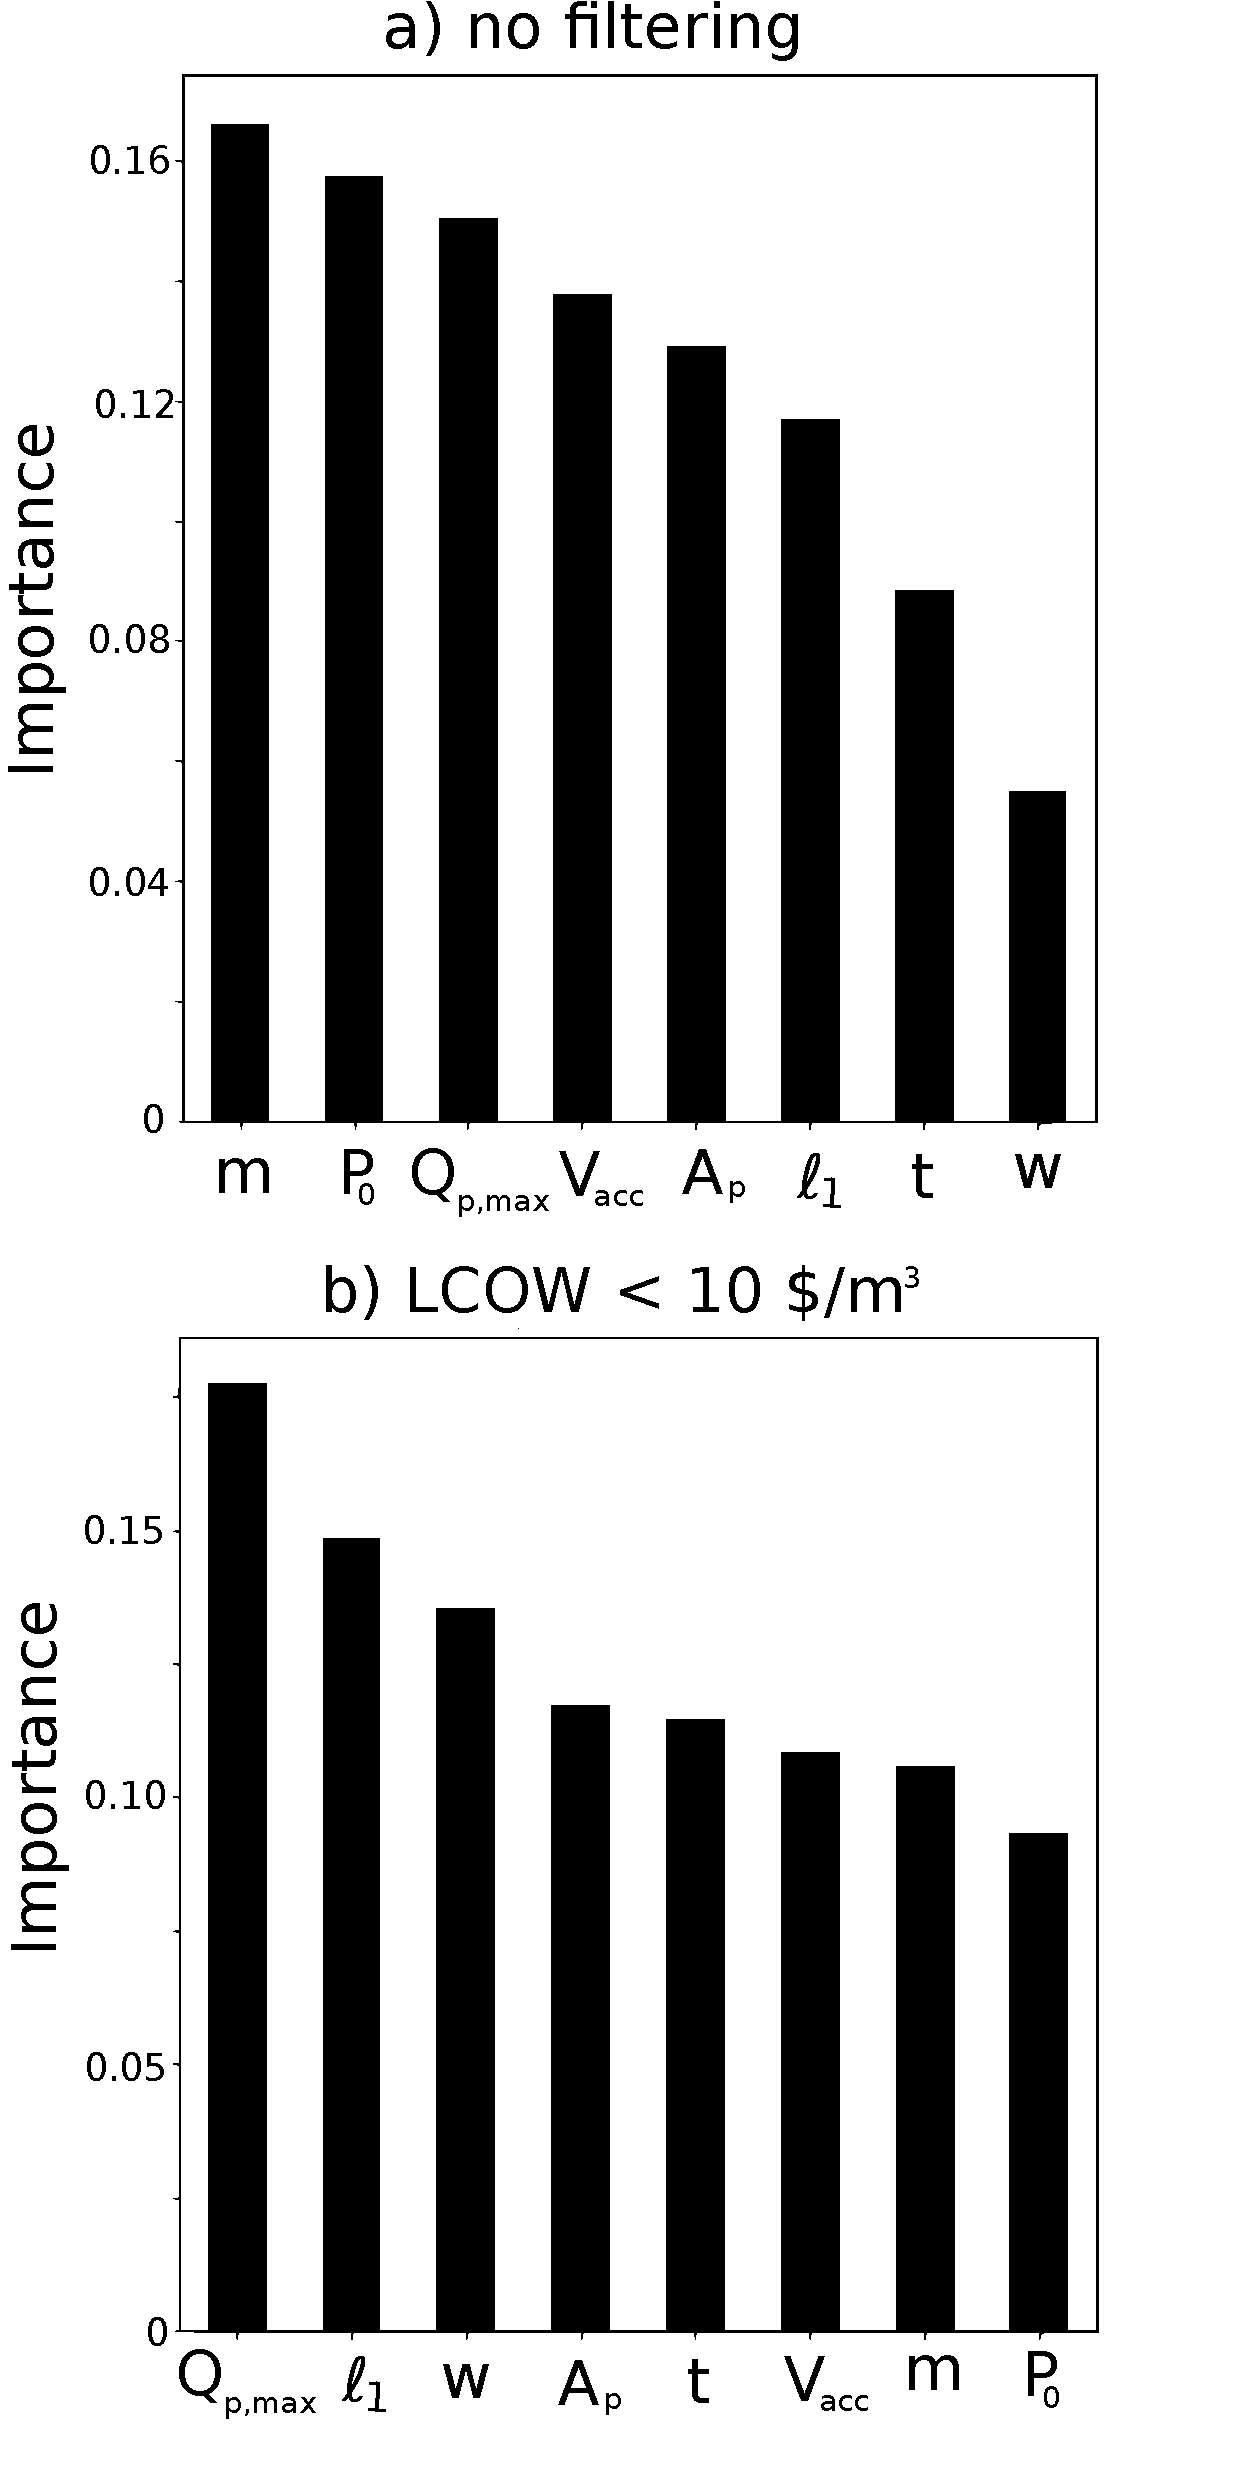
\includegraphics[width=0.6\linewidth]{../figs/importance.pdf}
    \captionof{figure}{Feature Importance of Design Variables. a) shows the importance when using the full dataset, b) shows the importance when using a filtered dataset with only design with an LCOW $<$ 10 \$/m$^3$ included, 338 out of 508 designs met this criteria. This allows us to compare importance for creating reasonable designs (a) as well as making reasonable designs better (b).}
    \label{fig:importance}
\end{figure}

\section{Discussion}
The DOE study reveals several key takeaways. The first takeaway is that the large disparity in LCOW values between the best and worst designs suggest substantial opportunities for optimization.  The minimum LCOW case (2.29~\$/m$^3$) is orders of magnitude lower than the maximum LCOW case (7547~\$/m$^3$), emphasizing the importance of design space exploration and optimization. 

The second takeaway is that poor system design can occur when WEC, PTO, and desalination plant capacities are mismatched. For example, the maximum LCOW case has a large WEC (24.5~m wide) and a large desalination plant capacity (9681~m$^3$/day), but an extremely small $\ell_1$ value (0.276~m). A small $\ell_1$ reduces the PTO's mechanical advantage, requiring excessive WEC motion to generate sufficient feedflow. A large WEC captures a high excitation torque from the waves and a large desalination plant requires significant feedwater flow to be cost-effective, making larger $\ell_1$ values essential. 

Other inefficient configurations could arise such as a large WEC and large PTO paired with a small desalination plant, leading to excess feedwater being wasted through the pressure relief valve, or a large PTO and desalination plant with a small WEC which lacks the wave capture potential necessary to drive the system efficiently. These findings reinforce the necessity of a holistic model approach---optimizing only one subsystem (e.g., WEC, PTO, or desalination plant) in insolation is insufficient.

The third takeaway is that the minimum LCOW case suggests a departure from conventional design trends in the literature. Specifically, the minimum LCOW design features a smaller accumulator volume (1.51 m$^3$) and a larger desalination capacity (7467 m$^3$/day). In contrast, previous studies have favored larger accumulators to smooth flucations in feedwater flow. Yu and Jenne used accumulator volumes of 4 m$^3$ (2018) and 6 m$^3$ (2017) for a 3150 m$^3$/day plant \cite{YJecon2017,Yu2018}. Brodersen et al. (2022) used a 6 m$^3$ accumulator for a 1700-2400 m$^3$/day desalination plant \cite{Brodersen2022}. These studies assumed that large accumulators improve feedwater regulation, allowing smaller desalination plants to capture a higher percentage of the flow. While this logic holds when ignoring accumulator costs, the DOE suggests that reducing accumulator volume and increasing desalination plant capacity can lead to a lower LCOW, further reinforcing the need for a holistic model when designing a WDDS.

Beyond cost savings, a smaller accumulator may also enhance system performance. Michelén Ströfer et al. (2022) demonstrated that a negative-stiffness PTO improves energy transfer for electricity-generating WECs  \cite{Stroefer2023}. The accumulator acts as a spring, where larger volumes correspond to higher effective stiffness. Therefore, a smaller accumulator (i.e., lower positive stiffness) may enhance energy transfer efficiency in the WDDS PTO.

The feature importance results indicate that all design variables have contribute significantly to LCOW prediction, suggesting that reducing design space dimensionality is not advisable. However, WEC mass and accumulator pre-charge pressure appear more important for ensuring reasonable designs than for refining optimal designs. Their importance decreases in the filtered dataset (Fig. \ref{fig:importance}b), suggesting that while they influence feasibility, they are less critical for improving already viable designs. This suggests that their bounds could be tightened, restricting low-performance regions while preserving design flexibility in promising designs. 

\section{Conclusion}
This study introduces an MDO framework for WDDS design. Preliminary DOE results suggest that MDO not only enhances system performance and but also influences  conventional design trends. Notably, our findings suggest that reducing accumulator sizes and increasing SWRO plant capacities can yield lower LCOE, a departure from prior WDDS assumptions.

The insights gained from this study underscore the importance of holistic optimization, as poor subsystem coordination---such as mismatched WEC, PTO, and desalination capacities---can result in inefficient and costly designs. The feature importance analysis further highlights the key design parameters that influence performance, paving the way for targeted refinements in future optimization studies.

Future work should focus on:
\begin{enumerate}
    \item Fully developing the PTO cost model by including piston and mechanism costs.
    \item Adding control to the system dynamics model, with de-clutching control \cite{Ringwood2014} identified as a particularly promising approach for WDDS.
    \item Comparing MDO results to those obtained through traditional sequential design optimization.
    \item Developing gradient-compatible models for the hydrodynamics and system dynamics modules to enable gradient-based optimization.
    \item Investigating different WDDS PTO architectures, such as incorporating an ERU, within this framework.
\end{enumerate}

The MDO framework presented in this study provides a systematic approach to optimizing WDDS, offering new pathways for improving desalination affordability and sustainability. Future advancements in control strategies, economic modeling, and real-world implementation will further strengthen the feasibility of wave-powered desalination as a scalable solution to global freshwater challenges.

\bibliographystyle{asmems4}
\bibliography{biblio}

\appendix
\newpage
\section{Tables of Parameters} \label{app:params}
\begin{table}[h]
    \centering
    \caption{General Parameters}
    \begin{tabular}{|c|c|c|}
        \hline
        \textbf{Parameter} & \textbf{Value} & \textbf{Units} \\
        \hline
        gravitational acceleration & 9.81 & m/s$^2$ \\
        ocean density & 1025 & kg/m$^3$ \\
        distance to shore & 500 & m \\
        ocean temperature & 298.15 & K \\
        water depth & 12 & m \\
        wave direction & 0 & degrees \\
        
        wave spectrum & Pierson–Moskowitz & -  \\
        significant wave height & 2.64 & m \\
        peak period & 9.86 & s \\

        Fixed Charge Rate & 10.8 & \% \\
        \hline
    \end{tabular}
    \label{tab:paramsgeneral}
\end{table}

\begin{table}[h]
    \centering
    \caption{SWRO Parameters}
    \begin{tabular}{|c|c|c|}
        \hline
        \textbf{Parameter} & \textbf{Value} & \textbf{Units} \\
        \hline
        feed flow total dissolved solids & 40000 & mg/L \\
        permeate flow total dissolved solids & 500 & mg/L \\
        salt molar weight & 58.44 & g/mol \\
        water permeability coefficient & $2.57\times10^{-12}$ & m$^3$/N-s \\
        recovery ratio & 51.5 & \% \\
        single unit membrane area & 35 & m$^2$ \\
        single unit permeate flow rate & 24.6 & m$^3$/day \\
        \hline
    \end{tabular}
    \label{tab:paramsswro}
\end{table}

\begin{table}[h]
    \centering
    \caption{WEC Parameters}
    \begin{tabular}{|c|c|c|}
        \hline
        \textbf{Parameter} & \textbf{Value} & \textbf{Units} \\
        \hline
        draft & 9 & m \\
        cg draft factor & -0.7778 & - \\
        unit inertia & 14.57 & m$^2$ \\
        RM5 surface area & 1214 & m$^2$ \\
        RM5 flap cost & 3364648.63 & \$ \\
        RM5 base cost & 1706415.27 & \$ \\
        RM5 bearings cost & 17420.34 & \$ \\
        RM5 mooring cost & 997819.2 & \$ \\
        RM5 monitoring cost & 616480.27 & \$/yr \\
        RM5 marine operations cost & 101387.23 & \$/yr \\
        RM5 shore operations cost & 347280.29 & \$/yr \\
        RM5 parts cost & 86237.2 & \$/yr \\
        RM5 consumables cost & 17480.19 & \$/yr \\
        RM5 insurance rate & 2 & \% \\
        \hline
    \end{tabular}
    \label{tab:paramswec}
\end{table}

\begin{table}[h]
    \centering
    \caption{Mechanism Parameters}
    \begin{tabular}{|c|c|c|}
        \hline
        \textbf{Parameter} & \textbf{Value} & \textbf{Units} \\
        \hline
        $\ell_2$ & 4.7 & m \\
        $\ell_3$ & 0 & m \\
        max piston stroke & 20 & m \\
        \hline
    \end{tabular}
    \label{tab:paramsmech}
\end{table}

\begin{table}[h]
    \centering
    \caption{Solver Parameters}
    \begin{tabular}{|c|c|c|}
        \hline
        \textbf{Parameter} & \textbf{Value} & \textbf{Units} \\
        \hline
        BEM frequencies & 0.2, 0.34, 0.48, ..., 3& rad/s \\
        SysDyn time step & 0.1 & s \\
        SysDyn sim time & 300 & s \\
        \hline
    \end{tabular}
    \label{tab:paramssolve}
\end{table}

\end{document}